\section{Distributed Octrees}

In this section we describe our software for the creation of octrees for the kiFMM in $\mathbb{R}^3$, Bempp-Tree\footnote{https://github.com/bempp/bempp-rs/tree/main/tree}. We've re-implemented optimal algorithms for the `bottom-up' construction of trees in parallel, whereby points distributed across each node are assembled into a parallel tree partitioned and load-balanced across a distributed system \cite{sundar2008bottom}. We demonstrate that on a single-node, our tree software performs well in comparison to leading single-node FMM codes \cite{wang2021exafmm}, where parallel experiments are omitted due to time constraints. In addition to good scaling, we leverage the power of Rust's Traits to write software that generalises across single-node and multi-node trees, allowing for users to implement single/multi-node fast algorithms with relative ease. We begin by describing in detail our method for constructing trees, following the discussion in \cite{sundar2008bottom} though we use an updated communication scheme in order to achieve a 2:1 balance based on more recent work in \cite{sundar2013hyksort}. We conclude with a short discussion on the communication intensive phases of the FMM in a distributed-memory FMM implementation, and how these can be addressed, as the next stage of this research project centers on the construction of a distributed memory kiFMM.

We make use of a standard space-filling curve known as a Morton encoding \cite{sundar2008bottom} to encode the boxes of an octree as described in Figure \ref{fig:chpt:3:sec:0:morton}. This approach encodes spatial locality in that boxes encoded in sorted Morton order correspond to a pre-order traversal of the corresponding octree. Once encoded the Morton encoding for a given box is referred to as a \textit{Morton key}. The main terminology which we will make use of with regards to trees created using Morton encodings are summarised Table \ref{table:chpt:3:sec:0:morton}.

Historically implementations of distributed memory octrees and quadtrees were `pointer based' \cite{tu2005scalable}. Starting with a random subset of points at each processor, each node would recursively refine its local octree until it arrived at level of recursion limited by a user defined constraint on the maximum number of particles in a leaf box. However this is complicated by the need to communicate and synchronise ancestor relationships across nodes. Furthermore as the point distribution is not generally known apriori, with each process controlling a local tree involving a subset of the initial points, reconciling local trees necessitates a global parallel merge. Overlapping boxes would result in the user defined constraint on the maximum number of particles per box being violated, necessitating further refinement. Further communication would then be required if a user requires a 2:1 balance. Finally, load-balancing to ensure each node has an approximately uniform weighting in terms of particles would be computed as a post processing step.

The significant complexities in implementing such trees has lead to softwares that rely on a `bottom up' approach, as opposed to a `top down' strategy as described above \cite{sampath2008dendro,BursteddeWilcoxGhattas11}. The basic strategies implemented here is to form a Morton encoding for points at each processor and use parallel sorts to ensure that each node contains a non-overlapping subset of the global tree. The Morton keys are kept only at the leaf level, with ancestor keys inferred to exist. These trees are therefore referred to as \textit{linear} trees, and have been shown to scale to trees created of tens of thousands of processors with billions of octants \cite{BursteddeWilcoxGhattas11}.

Beginning with point data distributed across $n_p$ nodes in a distributed memory system, our strategy for creating uniform and adaptive octrees is as follows,

\begin{enumerate}
    \item Generate a Morton key for each point at the leaf level corresponding to a user defined octree depth (uniform trees), or based on a critical value for the maximum number of points per leaf box (adaptive trees).
    \item Perform a parallel sort of these leaf octants, such that processors contain non-overlapping subsets of the global tree.
    \item \textit{Linearise} the leaves on each compute node, i.e. remove overlaps, favouring smaller leaves over larger ones. We use Algorithm \ref{alg:app:morton:linearise_octree} in Appendix \ref{app:morton} to do so.
    \item `Complete' the space defined by the largest and smallest leaf on each compute node. This amounts to finding the minimal octree that covers the region specified by the Morton keys at each process. This is described by Algorithm \ref{alg:app:morton:complete_region} in Appendix \ref{app:morton}. The coarsest boxes of this `complete' tree are referred to as `seeds'.
    \item Construct a `coarse block tree' by completing the space between seeds on each processor. The nodes of this tree are referred to as blocks, and help us to estimate the load balance of each compute node by calculating the number of original Morton keys they contain. This gives us a coarse distributed, complete, linear octree that is based on the underlying data distribution and contains load information.
    \item Point data is communicated to each compute nodes containing its associated block, and the blocks are refined based on the level of recursion defined by the user, which depends again on whether uniform or adaptive trees are requred. Providing the final, unbalanced, tree in the case of adaptive trees.
    \item For adaptive trees a 2:1 balance is computed on each subtree on each compute node using Algorithm \ref{alg:app:morton:balance_octree} in Appendix \ref{app:morton}. The locally balanced leaf octants can be sorted in parallel again, and locally linearised as in Step 3, to remove overlaps. Thus we are left with a globally balanced, linear, octree based on the original data distribution.
\end{enumerate}

This algorithm is summarised in Algorithm \ref{alg:app:morton:point2octree} in Appendix \ref{app:morton}. The complexity of this process is bounded by the parallel sorts, which for randomly distributed point data, run in $O(N_{\text{leaf}} \log (N_{\text{leaf}}))$ work and $O(\frac{N_{\text{leaf}}}{n_p} \log(\frac{N_{\text{leaf}}}{n_p}) + n_p \log (n_p))$ time where $N_{\text{leaf}}$ is the number of leaves in the final octree, and $n_p$ is the number of processors \cite{sundar2013hyksort}. This makes the efficiency of the parallel sort a bottleneck in tree construction.

\begin{figure}[h]
    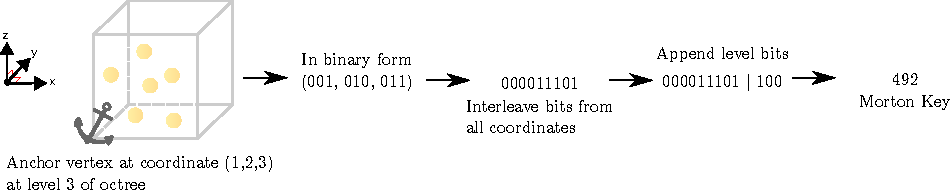
\includegraphics[width=\textwidth]{images/ch_3/morton.pdf}
    \caption{How to Morton encode a node in an octree. The node is described by an ‘anchor’ vertex, and its associated coordinate.}
    \label{fig:chpt:3:sec:0:morton}
\end{figure}


\begin{table}[h!]
\centering
\begin{tabular}{||c c||}
    \hline
    Relation & Definition \\ [0.5ex]
    \hline\hline
    Siblings($N$) & The seven (octree) or three (quadtree) Keys \\
        & that share a parent with $N$  \\
    Neighbours($N$) & Keys that share a face, edge, or vertex with $N$  \\
    Parent($N$) & The parent key of $N$  \\
    Children($N$) & The eight (octree) or four (quadtree) children of $N$  \\
    Descendants($N$) & All descendants of $N$  \\
    Ancestors($N$) & All ancestors of $N$  \\
    FinestAncestors($N$, $M$) & Finest shared ancestor of $N$ and $M$.  \\
    FirstChild($N$) & The `first', in Morton order, child of $N$  \\
    LastChild($N$) & The `last', in Morton order, child of $N$  \\
    DeepestFirstDescendant($N$) & The `first', in Morton order,  \\
        &  descendant of $N$ at the leaf level \\
    DeepestLastDescendant($N$) & The `last', in Morton order, \\
        & descendant of $N$ at the leaf level \\

    \hline
\end{tabular}
\caption{Definitions of Morton key relations for a given Morton key $N$.}
\label{table:chpt:3:sec:0:morton}
\end{table}

Designing and implementing an efficient sorting algorithm that can scale to thousands of cores is difficult since it requires irregular data access, communication, and equal load-balance. As first presented by Sundar et al, parallel sorts in the creation of octrees were implemented using a variant of Sample Sort \cite{sundar2008bottom}. Briefly, this approach samples elements at each processor to create a set of $n_p - 1 $ ordered `splitters', which are shared across all processors and define a set of $n_p$ buckets. This is followed by a global all-to-all communication call over all $n_p$ processors to assign elements to their corresponding bucket. Finally, a local sort is performed at each bucket to produce a globally sorted array. SampleSort is well understood. However, its performance is quite sensitive to the selection of splitters, which can result in load imbalance. Most importantly, the all-to-all key redistribution scales linearly with the number of tasks and can congest the network. As a result sample sort may scale sub-optimally, especially when the communication volume approaches the available hardware limits \cite{sundar2013hyksort}.

An alternative approach is provided by HykSort \cite{sundar2013hyksort}, which is a generalisation of Quicksort over a hypercube \cite{wagar1987hyperquicksort} from 2-way splits to $k$-way splits, with the addition of an optimised algorithm to select splitters. Quicksort, Hyksort and Sample Sort are compared in figure (\ref{fig:chpt:3:sec:0:hyksort}). Instead of splitting the global array into $n_p$ buckets, Hyksort splits it into $k < n_p$, and recursively sorts for each bucket. We notice that at each recursion step, each task communicates with just $k$ other tasks. Indeed, for $k=2$ we recover Quicksort over a hypercube. Both Hyksort, and the parallel splitter selection algorithm are provided in Appendix \ref{app:hyksort}, alongside complexity comparisons between Hyksort and Sample Sort. We note that Hyksort has a lower asymptotic complexity, with no terms that scale linearly in number of tasks in the MPI communicator, $p$, unlike Sample Sort.

\begin{figure}
    \centerline{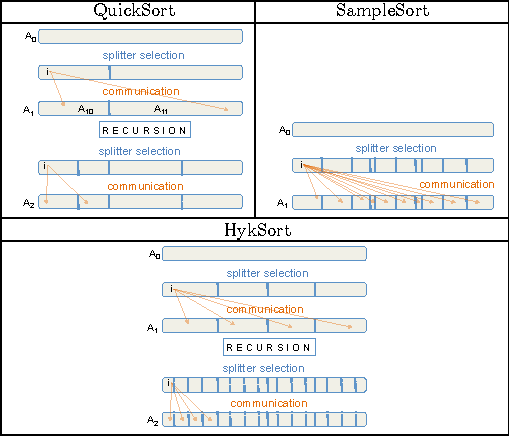
\includegraphics[width=0.7\linewidth]{images/ch_3/hyksort.pdf}}
    \caption{Communication pattern of Hyksort algorithm compared to a parallel Sample Sort, as well as a Quicksort over a hypercube, adapted from \cite{sundar2013hyksort}. We see that HykSort results in a lower communication overhead than Sample Sort.}
    \label{fig:chpt:3:sec:0:hyksort}
\end{figure}


Figure \ref{fig:chpt:3:sec:0:single_node_scaling} shows scaling of our software, `Bempp-Tree', on a single node as time limitations inhibited multi-node experiments. In the left figure compare the performance of linear trees constructed using our software with the pointer-based trees constructed using the functionality of ExaFMM-t the leading single-node implementation of the kiFMM. We limit this comparison to uniform trees as they don't offer adaptive functionality. In the right figure we show weak scaling for fixed 1e6 points per MPI process for adaptive and uniform trees. We observe that there is a constant overhead in constructing adaptive trees, this comes from having to recursively refine blocks from the block tree by counting how many points they contain. The significant jump when using 8 MPI processes is likely due to the number of MPI processes exceeding the number of cores available on the Intel i7-9750 processor used for the experiments. Our performance in the single-node case is excellent, where we're able to generate an octree with 8e6 points, with a depth of 5, in approximately 13.5s. A marked improvement over ExaFMM-T, and demonstrative of the power of a bottom up approach. Multi-node experiments are required to assess the performance of our library in comparison to other state of the art tree libraries \cite{sampath2008dendro,BursteddeWilcoxGhattas11}. However, as our approach closely follows theirs we don't expect performance to be significantly different.

\begin{figure}[h]
  \centering
  \begin{minipage}[b]{0.45\textwidth}
    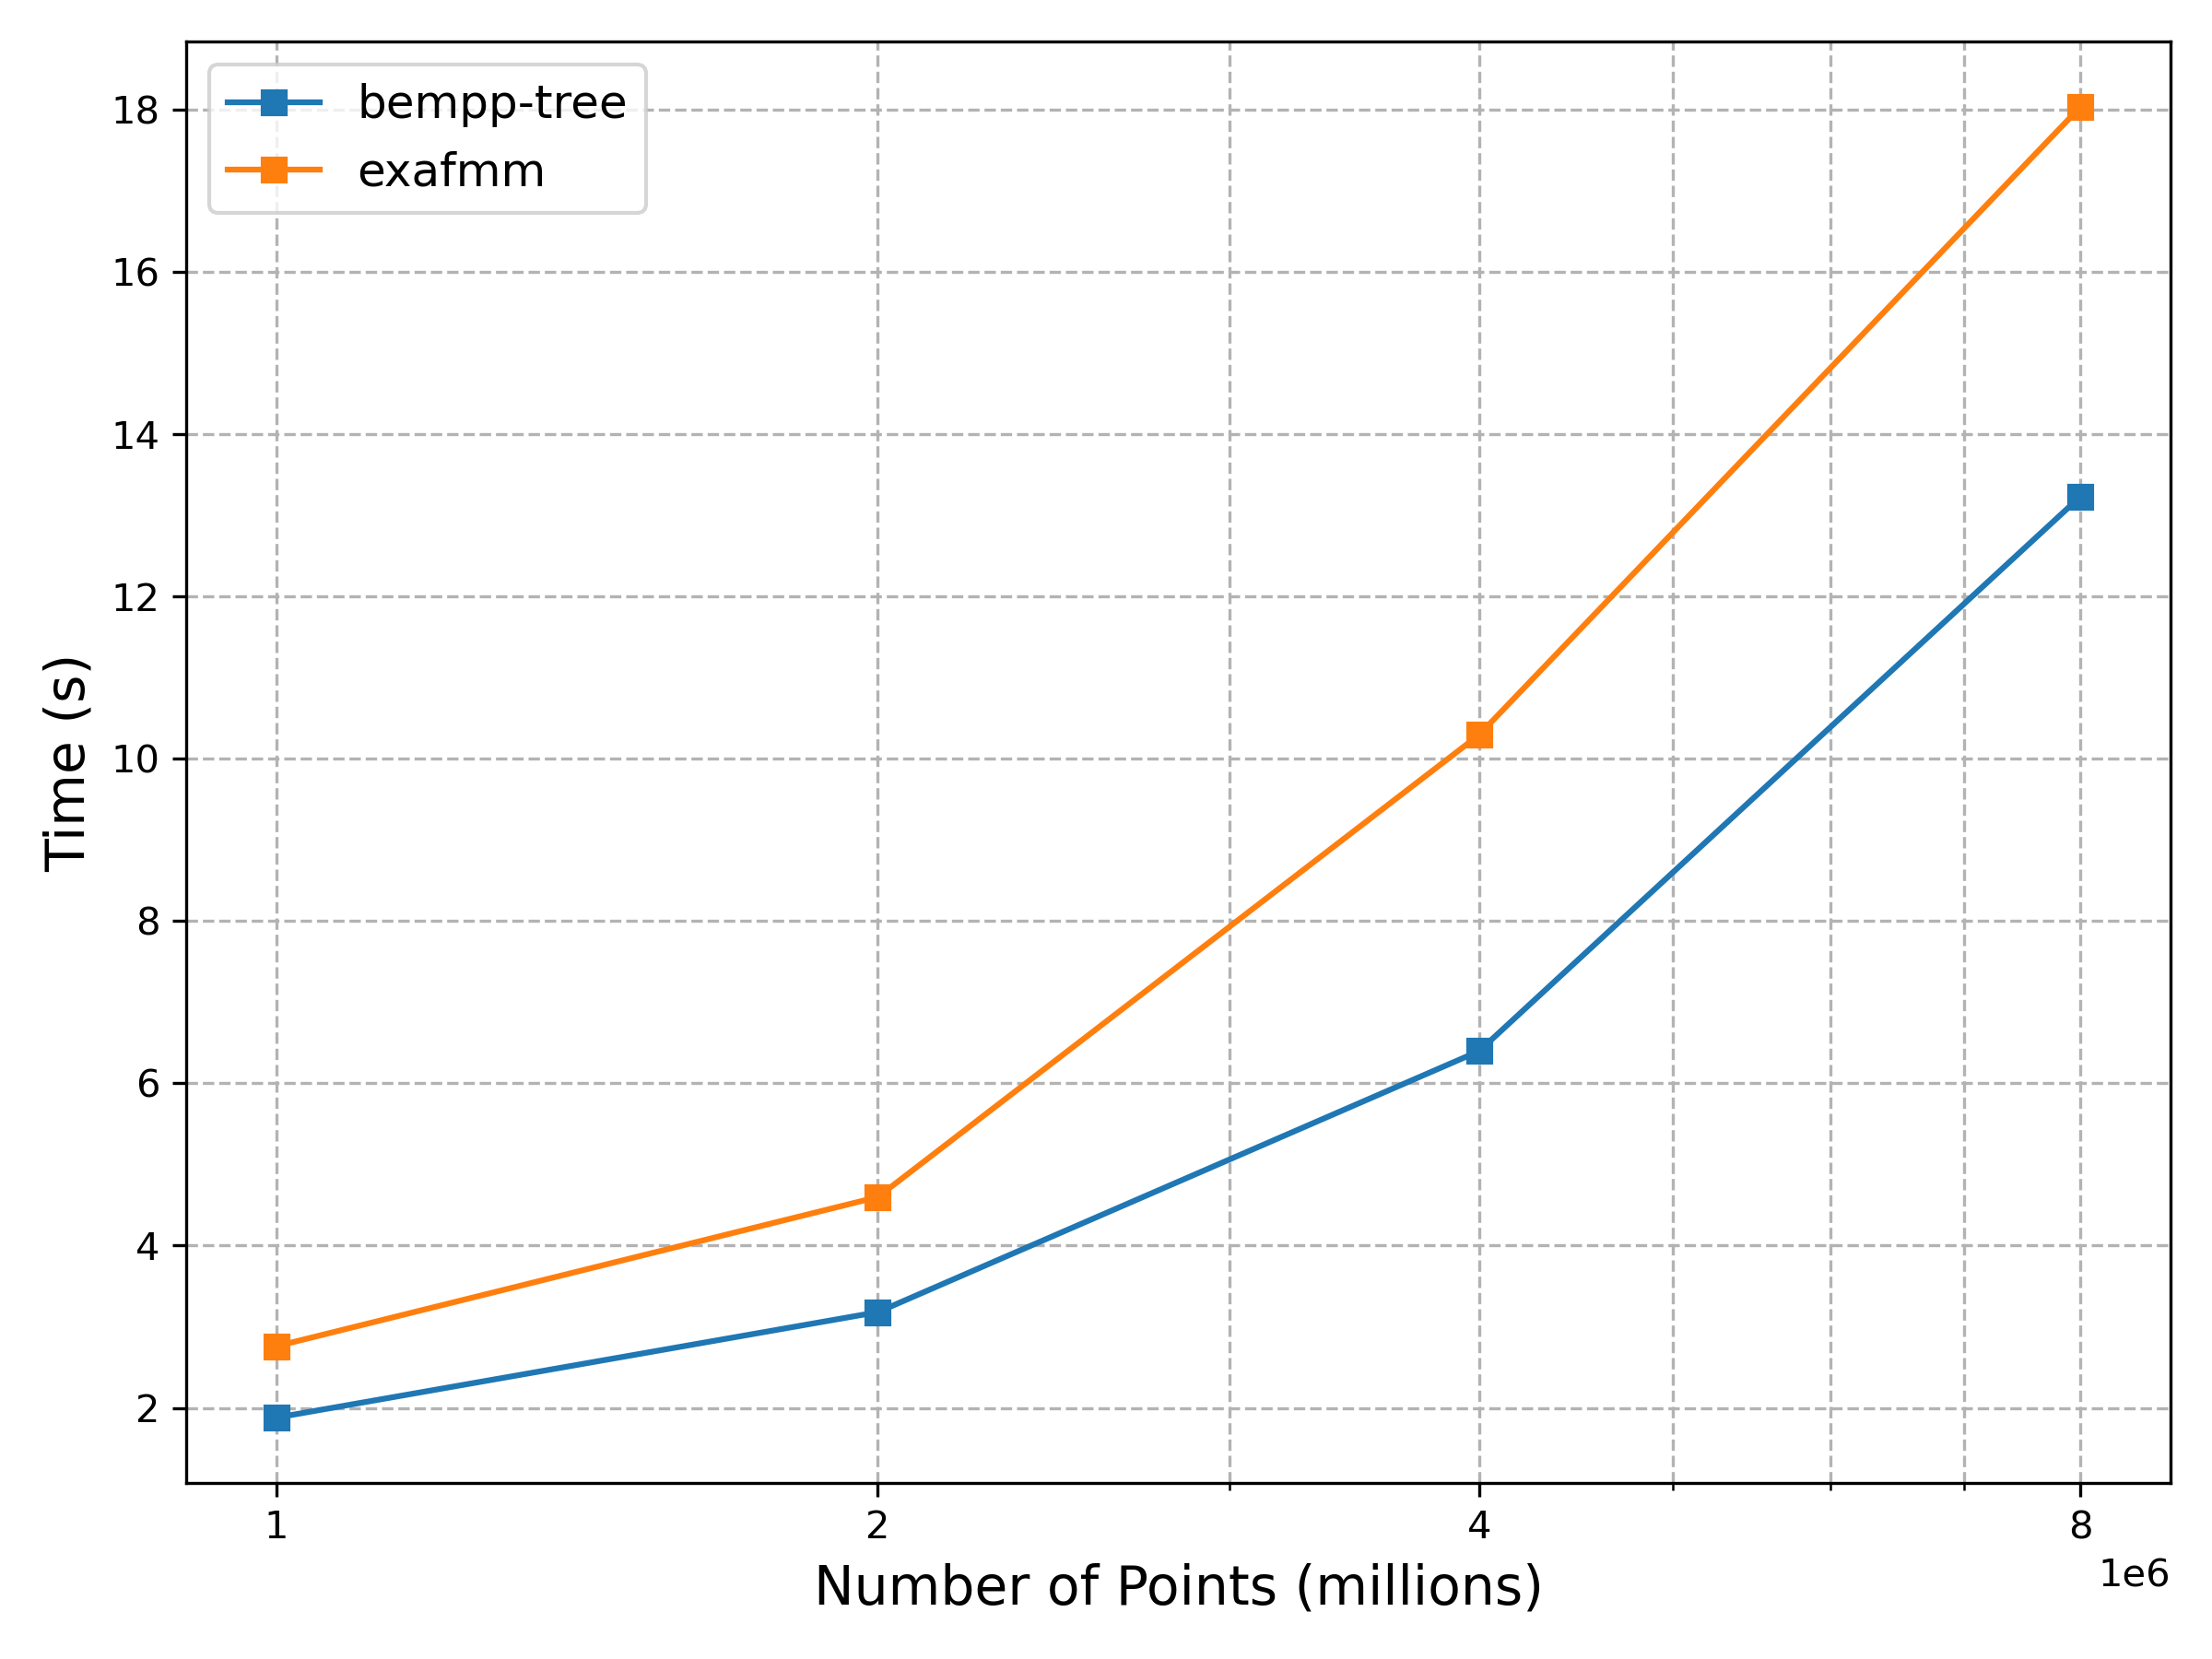
\includegraphics[width=\textwidth]{images/ch_3/single_node_scaling.png}
  \end{minipage}
  \hfill
  \begin{minipage}[b]{0.45\textwidth}
    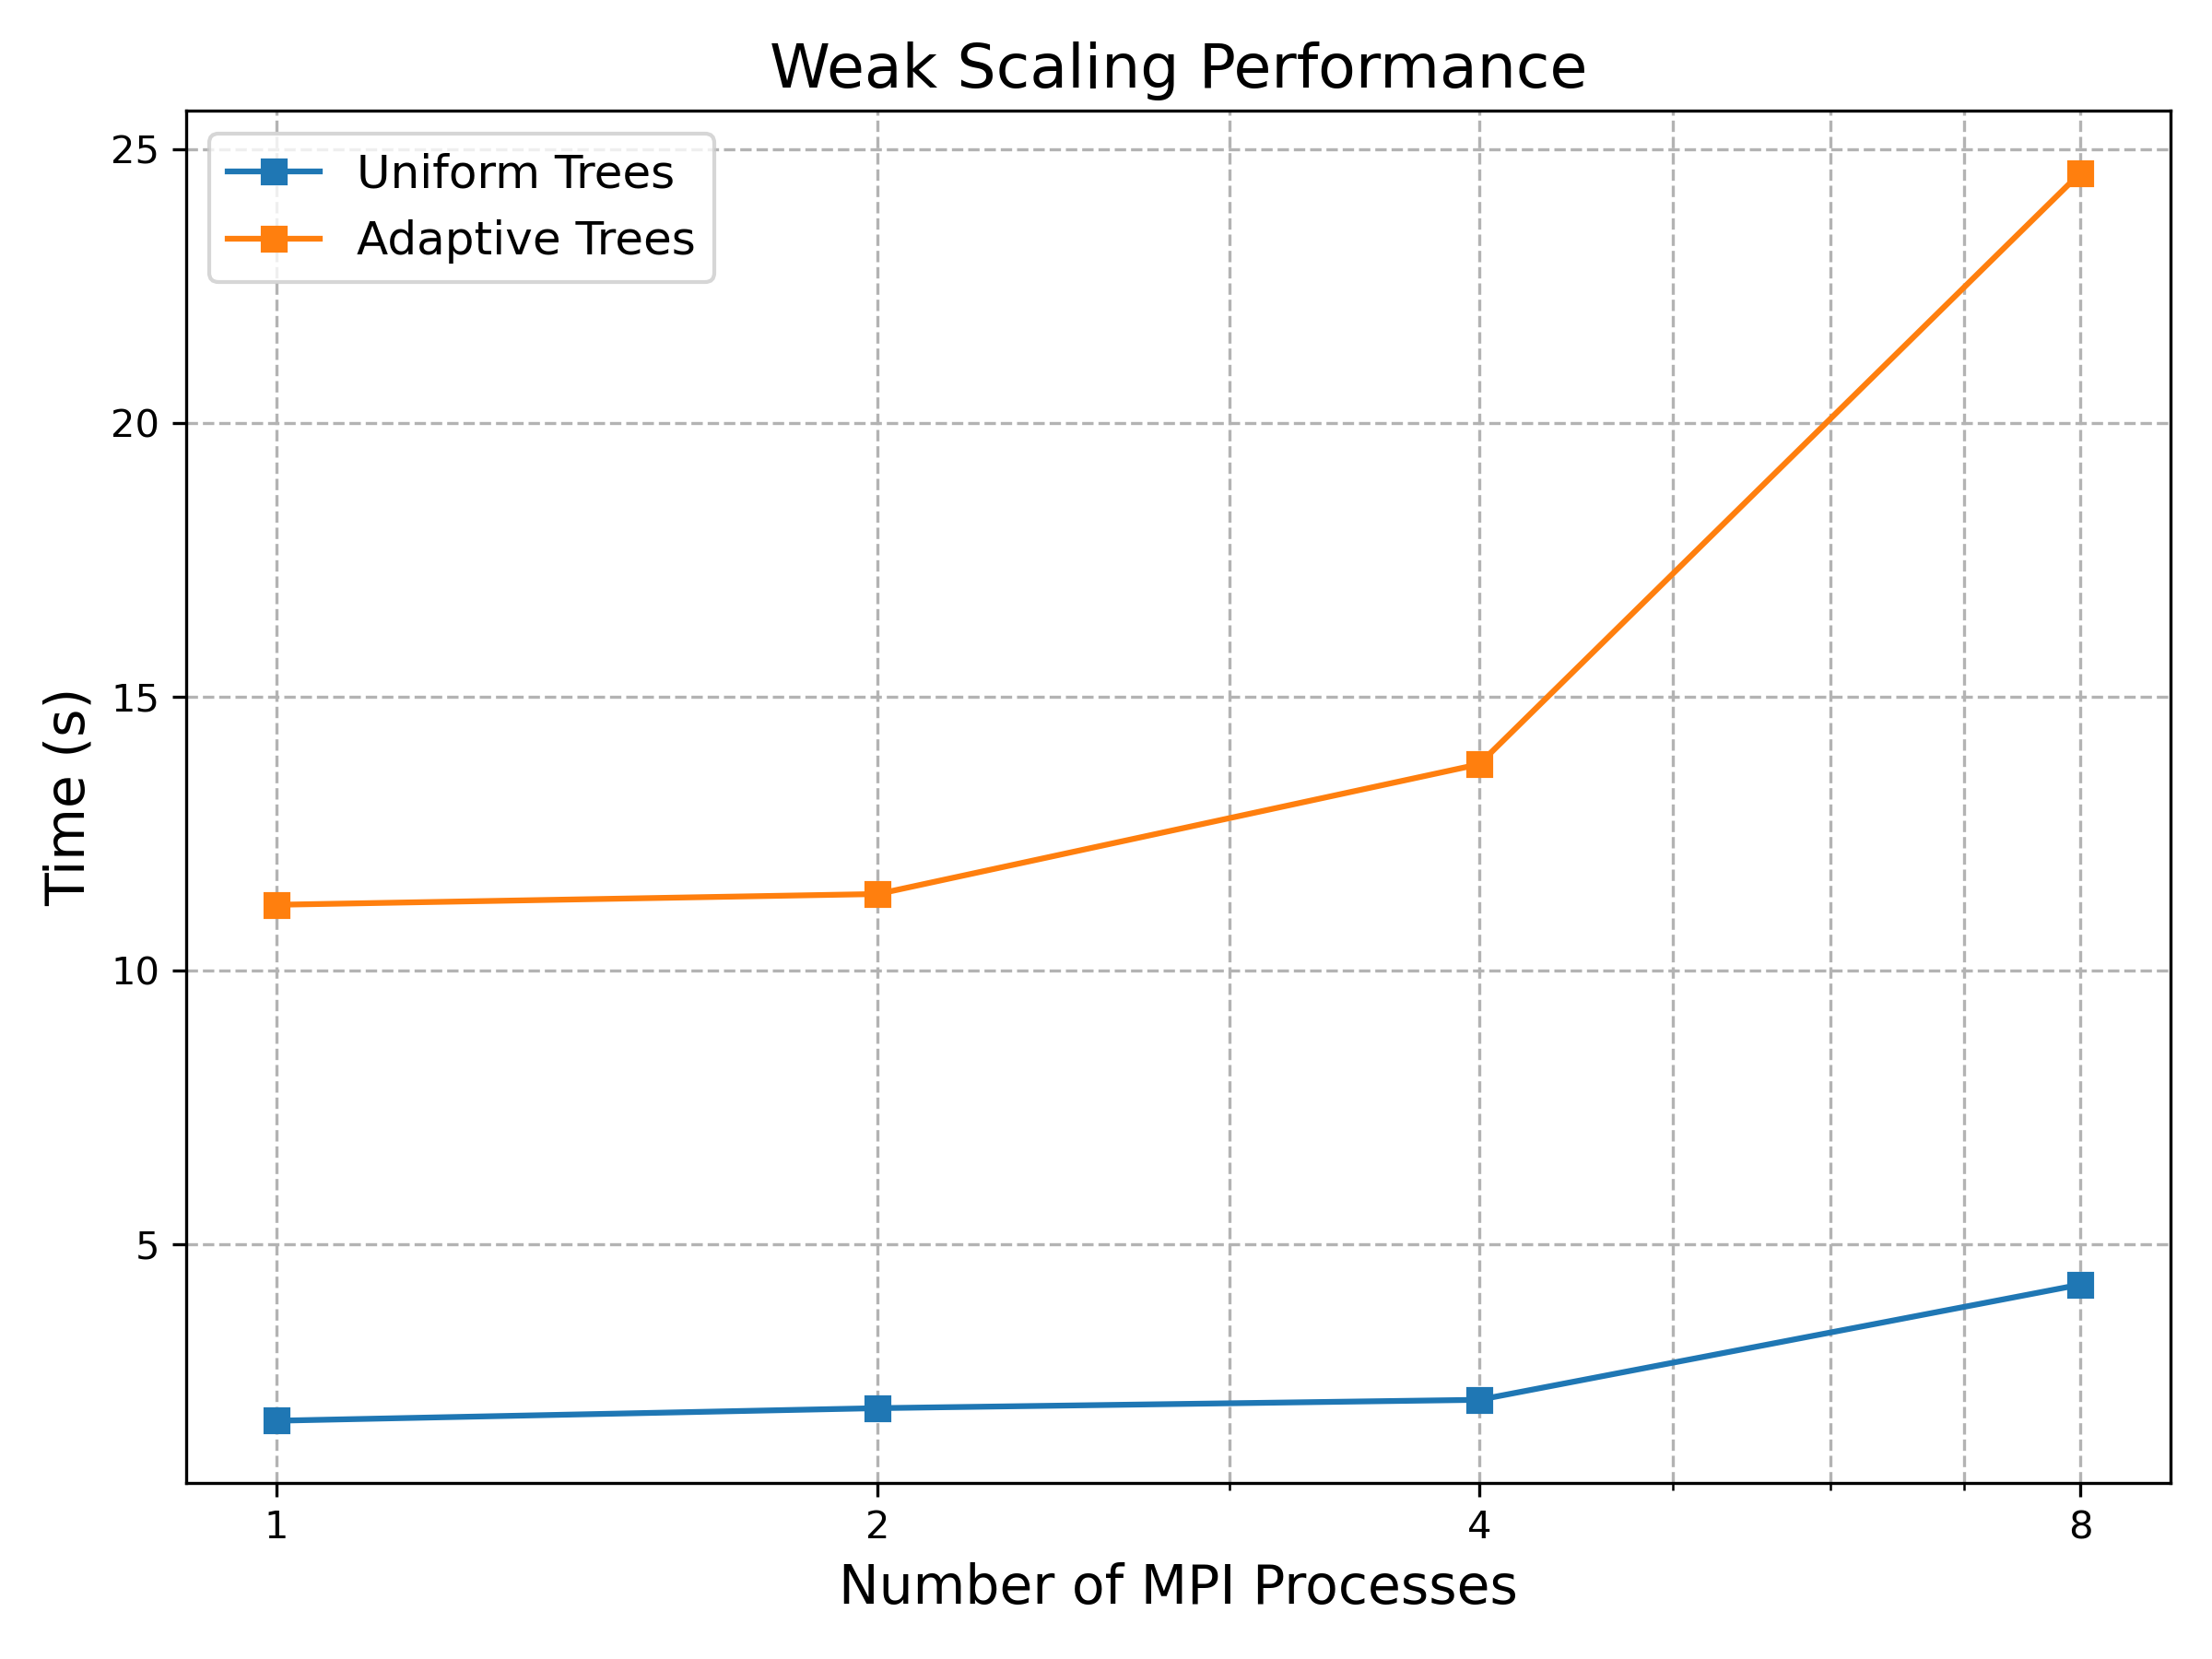
\includegraphics[width=\textwidth]{images/ch_3/weak_scaling_graph.png}
  \end{minipage}
\caption{The left figure shows the runtime of creating uniform trees on a single node in Bempp-Tree, in comparison to ExaFMM-T. The right figure shows weak scaling (over cores on a single node) of creating uniform and adaptive trees with Bempp-Tree, where each MPI process is given 1e6 points. The uniform trees are partitioned to a depth of 5, the adaptive trees have at most 150 particles in their leaf boxes. Experiments were taken on an Intel i7-9750H 6 core processor.}
\label{fig:chpt:3:sec:0:single_node_scaling}
\end{figure}

\subsection{Exposing Parallelism in A Distributed Memory FMM}

In the context of FMMs generating a distributed tree constitutes the first communication intensive phase. Further bottlenecks occur in the evaluation of the operators, most significantly in the evaluation of $T^{M2M}$ and $T^{M2L}$. To understand where these operators lead to communication bottlenecks, and how these can be overcome in practical implementations, we now introduce terminology relevant to distributing the FMM on parallel machines. We largely follow the discussion in Section 3 of \cite{Lashuk2012}, and use the same terminology.

Given a partition of a global tree $T$, as described above, such that each compute node $k$ contains a disjoint subset of leaves arranged in morton order, $T_k$m we define a \textit{Locally Essential Tree} (LET) for compute node $k$ as the union of interaction lists for all its owned leaves, as well as their ancestors,

\begin{flalign}
    \text{LET}(k) := \cup_{N \in T_k \cup \text{Ancestors}(T_k)} \text{InteractionList}(N)
    \label{eq:chpt:3:sec:0:let}
\end{flalign}

We denote the region controlled by compute-node $k$ as $\Omega_k$, from the properties of Morton keys (see app. \ref{app:morton}) this is defined by the smallest and largest Morton key they hold. Using an MPI\_AllGather collective, we exchange information about the bounds of each compute-node globally. Following this, ancestors are added to each $T_k$ for the leaf nodes they control. In order to communicate `ghost octants', i.e. octants which are relied upon by the translation operators acting upon each $T_k$ but are not held locally, we introduce the concept of `Contributor' and `User' compute nodes,

\begin{enumerate}
    \item Contributor compute nodes for an octant $N \in T$ are
    \[
        \mathcal{P}_c(N) := k \in 1...p : N \text{ overlaps with } \Omega_k
    \]
    \item User compute nodes of an octant $N \in T$ are
    \[
        \mathcal{P}_u(N) := k \in 1...p : \text{ Parent($N$) or Neighbours ($N$) overlaps with } \Omega_k
    \]
\end{enumerate}

We denote the set of octants which compute node $k$ contributes and which process $k'$ uses as $I_{k k'}$. These are communicated and inserted into each compute node's local tree in order to complete the construction of its LET. Consider the potential generated by the sources enclosed by some octant $N$. In order to evaluate the potential outside the volume covered by $\text{Neighbours}(\text{Parent})(N)$ one doesn't need the multipole expansions, or sources, associated with $N$ as an ancestor of $N$ would be used instead. This ensures the correctness of this approach to constructing LETs.

During evaluation of the FMM Lashuk et. al define three communication phases.

\dots

Ibeid et. al demonstrate a communication scheme with a reduced complexity bound.

\dots



- Data dependencies of the FMM  - P2M and U list have no dependencies on anything else
    - one can pipeline p2m, m2m and m2l steps to expose more parallelism
    - one strategy is to use MPI based global tree andpartition into overlapping subtres LETs to remove data dependencies between m2l and x list, as well a w list and l2p
    - define LET
        - for a process k the LET is the union of interaction lists for all owned leaves and their ancestors.
        - once constructed can run the FMM in parallel over each processor.
            - two comm intesnive, first is LET construction
            - second is all-reduce during evaluation?

    - LET construction
        - MPI all gather to exchange region contrlled by each processor
        - add all ancestor octants to local leaves, creating LET
        - exchange ghost octants using comm scheme, ghosts are exchanged for leaves and non-leaves.
        - repartition to get equal load.

    - Evaluation
        - pre M2M
            - first step
            - communicate source charges required for near field interaction.
                - MPI Isend - relatively local communicatons
        - M2M
            - second step, sum up multipoles o the contributors to each octant.
            - third step, communicate th collected upward densities to uses of each octant, as they only have a part of the final sum.
        - second and third steps same as allreduce  on a hypercube.

- How must we break down the communication pattern during this algorithm to achieve optimal communication bound of the FMM? (global vs local tree)?


It is a near term priority of this research project to combine the enhanced communication scheme proposed by Ibeid et. al. with the LET construction of Lashuk et. al. in our implementation.

